\documentclass{beamer}

\usepackage[utf8x]{inputenc}
\usepackage{default}
\usepackage[T1]{fontenc}
\usepackage[ngerman]{babel}
\usepackage{pgf}
\usepackage{tikz}
\usetikzlibrary{arrows,automata}
\usepackage[german]{fancyref}
\usepackage{float}
\usepackage{wrapfig}
\hyphenation{Ver-bund-wahr-schein-lich-keits-ver-tei-lung}

\title{Vergleich Probabilistischer Graphischer Modelle}
\author{Bernhard Häussner}
\date{18. Juni 2013}

\begin{document}


\maketitle
 
\section{Einführung}
\frame{\tableofcontents[currentsection]}

\begin{frame}
  \frametitle{Probabilistische graphische Modelle (PGM)}
  \begin{itemize}
    \item Interdisziplinär: Computer Vision, medizinische Entscheidungsfindung...
    \item Beginn in Expertensystemen
    \item Heute im Rahmen des Web 2.0
    \item Aus Profildaten in sozialen Netzwerken, Nutzungsprofile in Onlineshops...
    \item ...Produktempfehlungen, Spamfilter
  \end{itemize}
\end{frame}

\begin{frame}
  \frametitle{Definition probabilistisches graphisches Modell}
  \begin{itemize}
    \item Datenstruktur für eine gemeinsame Wahrscheinlichkeitsverteilung
    \item $P(X_1, X_2, ... X_n)$ über viele Zufallsvariablen $X_1,X_2,\dots,X_n$ 
    \item n meistens zwischen 5-100
    \item Grad an Unsicherheit 
    \item Graphen mit Wahrscheinlichkeitsverteilungen
  \end{itemize}
\end{frame}

\begin{frame}
  \frametitle{Warum probabilistische graphische Modelle?}
  \begin{itemize}
    \item $P(X_1, ..., X_n)$ hat exponentiell viele Werte
    \item Für jede mögliche Belegung der Variablen einen
    \item z.B. $30$ binäre Zufallsvariablen $\rightarrow$ $2^{30} \approx 10^9 $ Werte
    \item Benötigter Speicherplatz sehr groß
    \item Einzelne Wahrscheinlichkeiten sehr klein
  \end{itemize}
\end{frame}


\begin{frame}
  \frametitle{Workflow bei probabilistischen graphischen Modellen}
  \begin{itemize}
    \item Automatisches Lernen aus Stichproben 
    \item Mit Modell Beschaffenheit der Testobjekte analysieren
    \item Oder: direkt von Domainexperten erstellt werden. 
    \item Dann Schließen mit Inferenzalgorithmen
    \item Wahrscheinlichkeitsverteilungen für Zielvariablen
  \end{itemize}
\end{frame}

\begin{frame}
  \frametitle{Beispiel}
  \begin{figure}[htb]
  \caption{\label{fig:bayesnetwork}Beispiel für ein bayessches Netz zum Thema Pilze}
  \centering
  \begin{tikzpicture}
    %[->,>=stealth',shorten >=1pt,auto=left,every node/.style={circle,draw}]
    [scale=0.6,->,>=stealth',shorten >=1pt,auto=left,every node/.style={circle,draw}]
    \node (nf) at (2,4) {Farbe};
    \node (nm) at (6,4)  {Muster};
    \node (ng) at (4,1)  {Gift};

    \path (nf) edge (nm);
    \path (nf) edge (ng);
    \path (nm) edge (ng);

  \end{tikzpicture}
  \end{figure}
\end{frame}

\section{Naive Bayesmodelle}
\frame{\tableofcontents[currentsection]}

\begin{frame}
  \frametitle{Beispiel für ein naives Bayesmodell}
  \begin{figure}[htb]
  \caption{\label{fig:nbgraph}Beispiel für ein naives Bayesmodell}
  \centering
  \begin{tikzpicture}
    %[->,>=stealth',shorten >=1pt,auto=left,every node/.style={circle,draw}]
    [scale=0.8,->,>=stealth',shorten >=1pt,auto=left,every node/.style={circle,draw,scale=0.8}]
    \node (nc) at (2.5,2.5) {$C$};
    \node (nf) at (1,1) {Farbe};
    \node (nm) at (2.5,1)  {Muster};
    \node (ng) at (4,1)  {Gift};

    \path (nc) edge (nf);
    \path (nc) edge (ng);
    \path (nc) edge (nm);

  \end{tikzpicture}
  \end{figure}
\end{frame}

\begin{frame}
  \frametitle{Beschreibung naiver Bayesmodelle}
  \begin{itemize}
    \item Konstruktion einer unbeobachtbaren Zufallsvariable $C$
    \item Zustände von $C$ heißen Klasse oder Komponente
    \item Annahme: In Abhängigkeit von $C$ alle Zufallsvariablen unabhängig
    \item Einfaches baumförmiges bayessches Netz mit $C$ als Wurzel
    \item Faktorisierung der Wahrscheinlichkeitsverteilung: 
\[ P(C,X_1,X_2,\dots,X_n) = P(C) \prod_{i=1}^n P(X_i|C) \]
  \end{itemize}
\end{frame}




\section{Probabilistische Entscheidungsgraphen}
\frame{\tableofcontents[currentsection]}

\begin{frame}
  \frametitle{Beschreibung probabilistischer Entscheidungsgraphen (1)}
  \begin{itemize}
    \item Nicht auf Unabhängigkeiten zwischen Zufallsvariablen basiert
    \item Zwei kaskadierende Graphen
    \item Wald mit Knoten für Zufallsvariablen $P(X_1,X_2,\dots,X_n)$ und baumförmigen Abhängigkeiten
    \item Verbundwahrscheinlichkeit je eines Baumes unabhängig
    \item Zweiter Graph mit Wahrscheinlichkeiten
  \end{itemize}
\end{frame}

\begin{frame}
  \frametitle{Beschreibung probabilistischer Entscheidungsgraphen (2)}
  \begin{itemize}
    \item Knotenmengen $V_i$ für jede Zufallsvariable $X_i$
    \item Für jeden möglichen Wert von $X_i$ genau eine Kante
    \item Zu einem Knoten aus $V_l$ (Nachfolger $X_l$ von $X_i$ im Wald)
    \item Jeder Knoten $v_{i,k} \in V_i$ annotiert mit Wahrscheinlichkeitsverteilung $P_{i,k}(X_i)$
    \item Verbundwahrscheinlichkeitsverteilung in Abhängigkeit der durch Variablenbelegung erreichten Knoten: 
\[P(x_1,x_2,\dots,x_n) = \prod_{i=1}^n P_{i,k}(x_i) \]
  \end{itemize}
\end{frame}

\begin{frame}
  \frametitle{Beispiel für einen probabilistischen Entscheidungsgraphen}
  \begin{figure}[H]
  \caption{\label{fig:pdgforest}Beispiel für den Abhängigkeiten-Wald eines probabilistischen Entscheidungsgraphen}
  \centering
  \begin{tikzpicture}
    %[->,>=stealth',shorten >=1pt,auto=left,every node/.style={circle,draw}]
    [scale=0.9,->,>=stealth',shorten >=1pt,auto=left,every node/.style={circle,draw}]
    \node (nf) at (1,3) {Farbe};
    \node (nm) at (3,2)  {Muster};
    \node (ng) at (1,1)  {Gift};

    \path (nf) edge (nm);
    \path (nm) edge (ng);

  \end{tikzpicture}
  \end{figure}
\end{frame}

\begin{frame}
  \frametitle{Beispiel für den gewurzelten azyklischen Graphen eines probabilistischen Entscheidungsgraphen}
  \begin{figure}[H]
  \centering
  \begin{tikzpicture}
    [scale=0.7,->,>=stealth',shorten >=1pt,auto=left,every node/.style={align=center,scale=0.7}]
    \tikzstyle{every state}=[circle,draw]
    \begin{scope}
      \draw[black, dashed, thin] (10,8) rectangle (7,6);
      \fill[black] (9.5,7) node[scale=1.2] {$V_F$};
      \node[state] (f1) at (8,7) {$v_{\text{Farbe},1}$ \\ $0,6/0,4$};
    \end{scope}
    \begin{scope}
      \draw[black, dashed, thin] (5,3) rectangle (11,5);
      \fill[black] (8,4) node[scale=1.2] {$V_\text{Muster}$};
      \node[state] (m1) at (6,4) {$v_{\text{Muster},1}$ \\ $0,9/0,1$};
      \node[state] (m2) at (10,4) {$v_{\text{Muster},2}$ \\ $0,3/0,7$};
    \end{scope}
    \begin{scope}
      \draw[black, dashed, thin] (3,0) rectangle (13,2); 
      \fill[black] (10,1) node[scale=1.2] {$V_\text{Gift}$};
      \node[state] (g1) at (4,1) {$v_{\text{Gift},1}$ \\ $1,0/0,0$};
      \node[state] (g2) at (8,1) {$v_{\text{Gift},2}$ \\ $0,5/0,5$};
      \node[state] (g3) at (12,1) {$v_{\text{Gift},3}$ \\ $0,0/1,0$};
    \end{scope}

    \path (f1) edge node {braun} (m1);
    \path (f1) edge node {rot} (m2);
    \path (m1) edge node {keines} (g1);
    \path (m1) edge node {weiße Tupfen} (g2);
    \path (m2) edge node {keines} (g2);
    \path (m2) edge node {weiße Tupfen} (g3);

  \end{tikzpicture}
  \end{figure}
\end{frame}

\begin{frame}
  \frametitle{Charakterisierung probabilistischer Entscheidungsgraphen}
  \begin{itemize}
    \item Teilt die Verbundwahrscheinlichkeit sehr übersichtlich auf
    \item Partitionen des Zustandsraums der Zufallsvariablen
    \item Schließen in linearer Zeit
    \item Unabhängigkeiten in bayesschen Netzen, die nicht mit probabilistischen Entscheidungsgraphen repräsentiert werden können
    \item Inkompatibel mit bayesschen Netzen
  \end{itemize}
\end{frame}


\section{Vergleich der PGMs}
\frame{\tableofcontents[currentsection]}

\begin{frame}
  \frametitle{Vergleich am Expertensystem}
  \begin{itemize}
    \item Welche der drei Methoden ist die beste?
    \item Expertensysteme für medizinische Diagnosen in zwei Versionen
    \item Frühere Version, mit naiven Bayesmodellen, 47/53 Fälle richtig
    \item Spätere Version,mit bayesschen Netzwerken, 50/53 Fälle richtig
    \item naive Bayesmodelle schlechter?
  \end{itemize}
\end{frame}

\begin{frame}
  \frametitle{Vergleich mit vielen Daten}
  \begin{itemize}
    \item 50 Datensätze aus dem UCI Machine Learning Repository
    \item NB teils genauer, teils an­nä­hernd gleich genau
    \item Inferenz deutlich schneller
    \item NB sehr leicht zu implementieren ($2500$ LOC)
    \item naive Bayesmodelle besser?
  \end{itemize}
\end{frame}

\begin{frame}
  \frametitle{Vergleich mit probabilistischen Entscheidungsgraphen}
  \begin{itemize}
    \item Was ist mit probabilistischen Entscheidungsgraphen?
    \item $\rightarrow$ Nielsen und Jaeger, 2006
    \item Vergleich mit 5 festen Lern- und Vergleichsdatensätzen
    \item Genauigkeit mit logarithmierter Likelihood-Funktion gemessen
    \item Vergleich mit Größe des Modells $\rightarrow$ Effizienz
  \end{itemize}
\end{frame}

\begin{frame}
  \frametitle{Systematik des Vergleich}
  \begin{itemize}
    \item Automatisches Lernen mit Lerndaten
    \item Vergleich mit (anderen) Vergleichsdaten
    \item Gleiche Daten für alle drei Methoden
    \item Auftragen in Diagrammen mit SL-Kurven
  \end{itemize}
\end{frame}

\begin{frame}
  \frametitle{Ausschnitt der SL-Kurven aus den Daten von Nielsen und Jaeger}
  \begin{figure}[H]
    \caption{\label{fig:datagraphs}SL-Kurven mit empirischen Daten von Nielsen und Jaeger}
    \centering
    %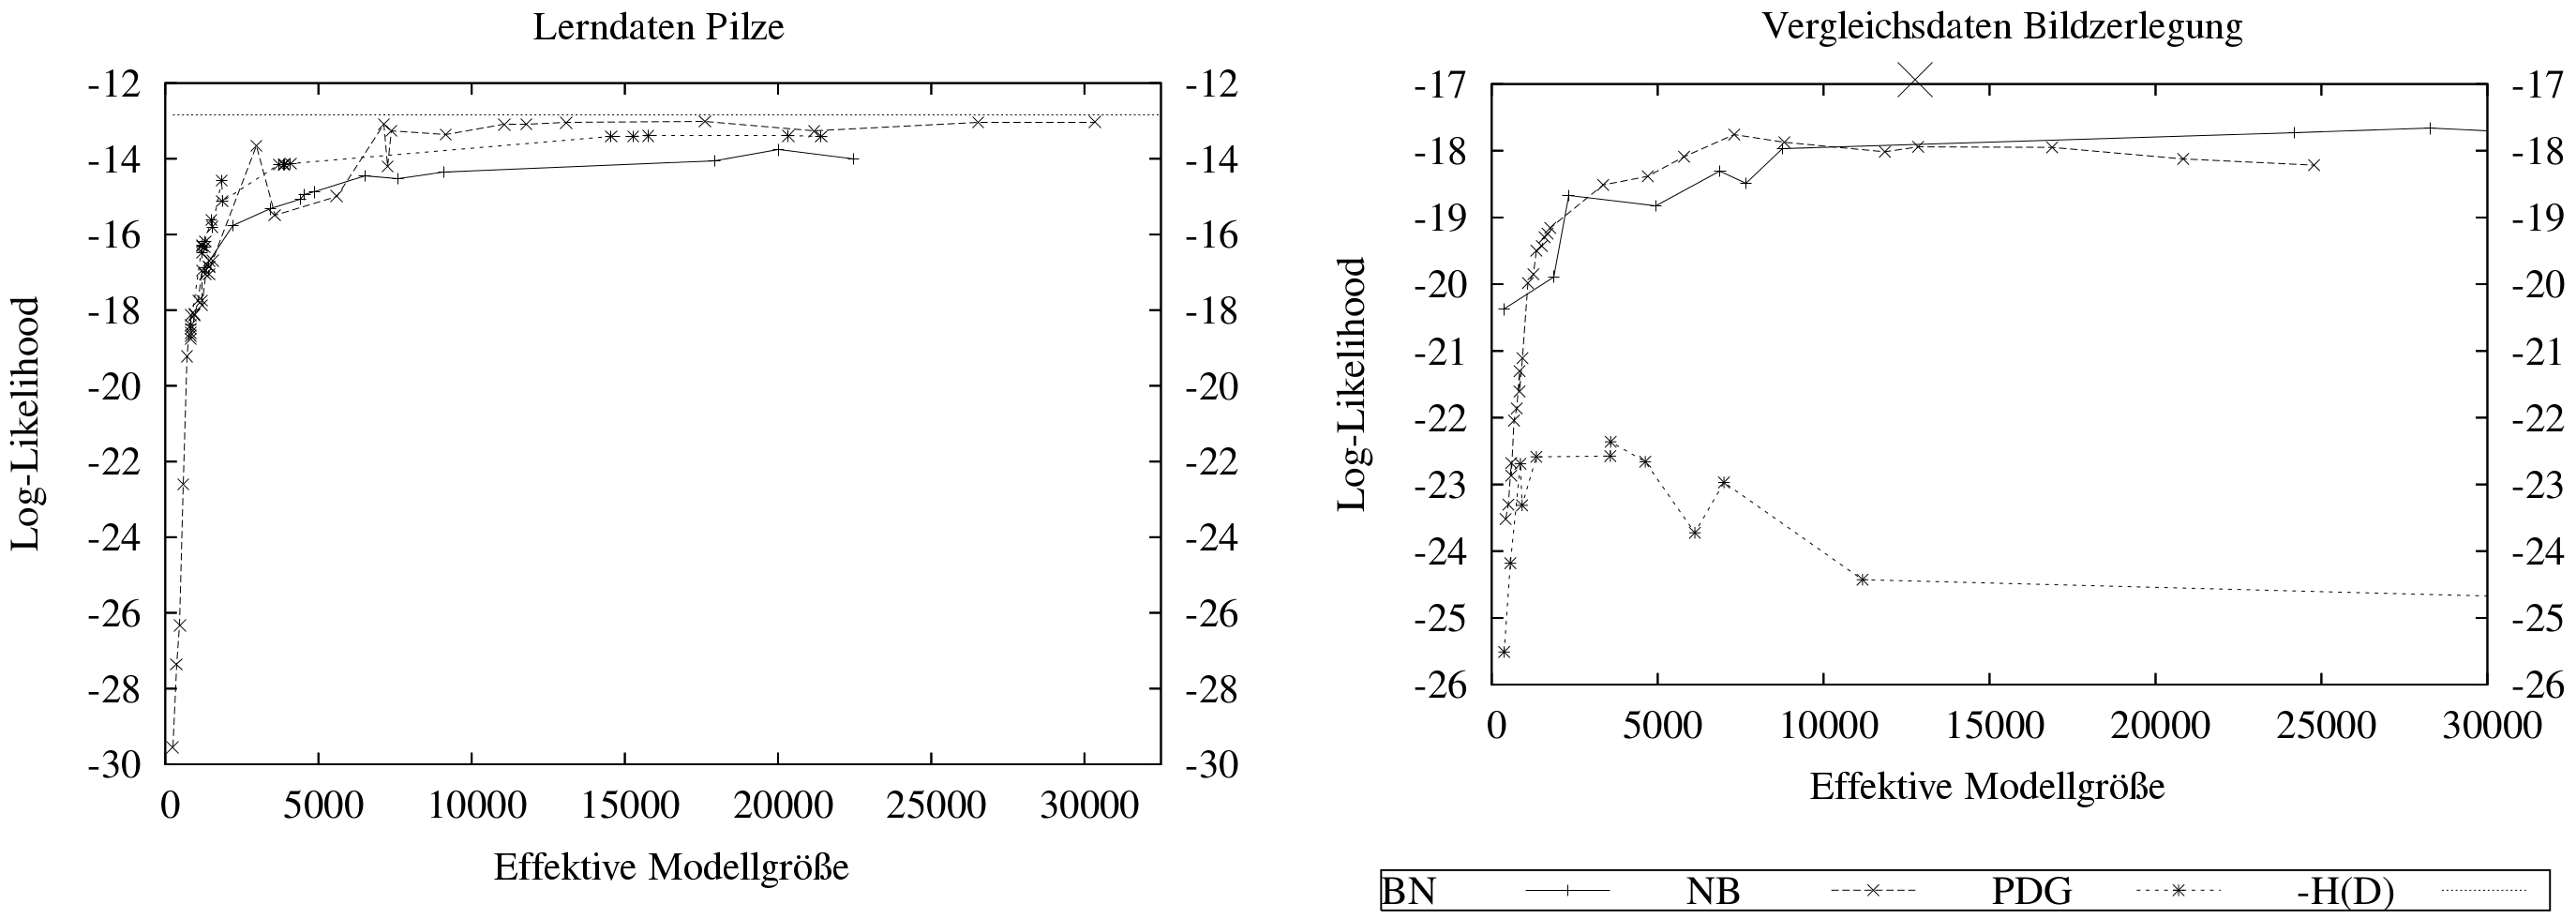
\includegraphics[width=0.7\textwidth]{graphs.png}
    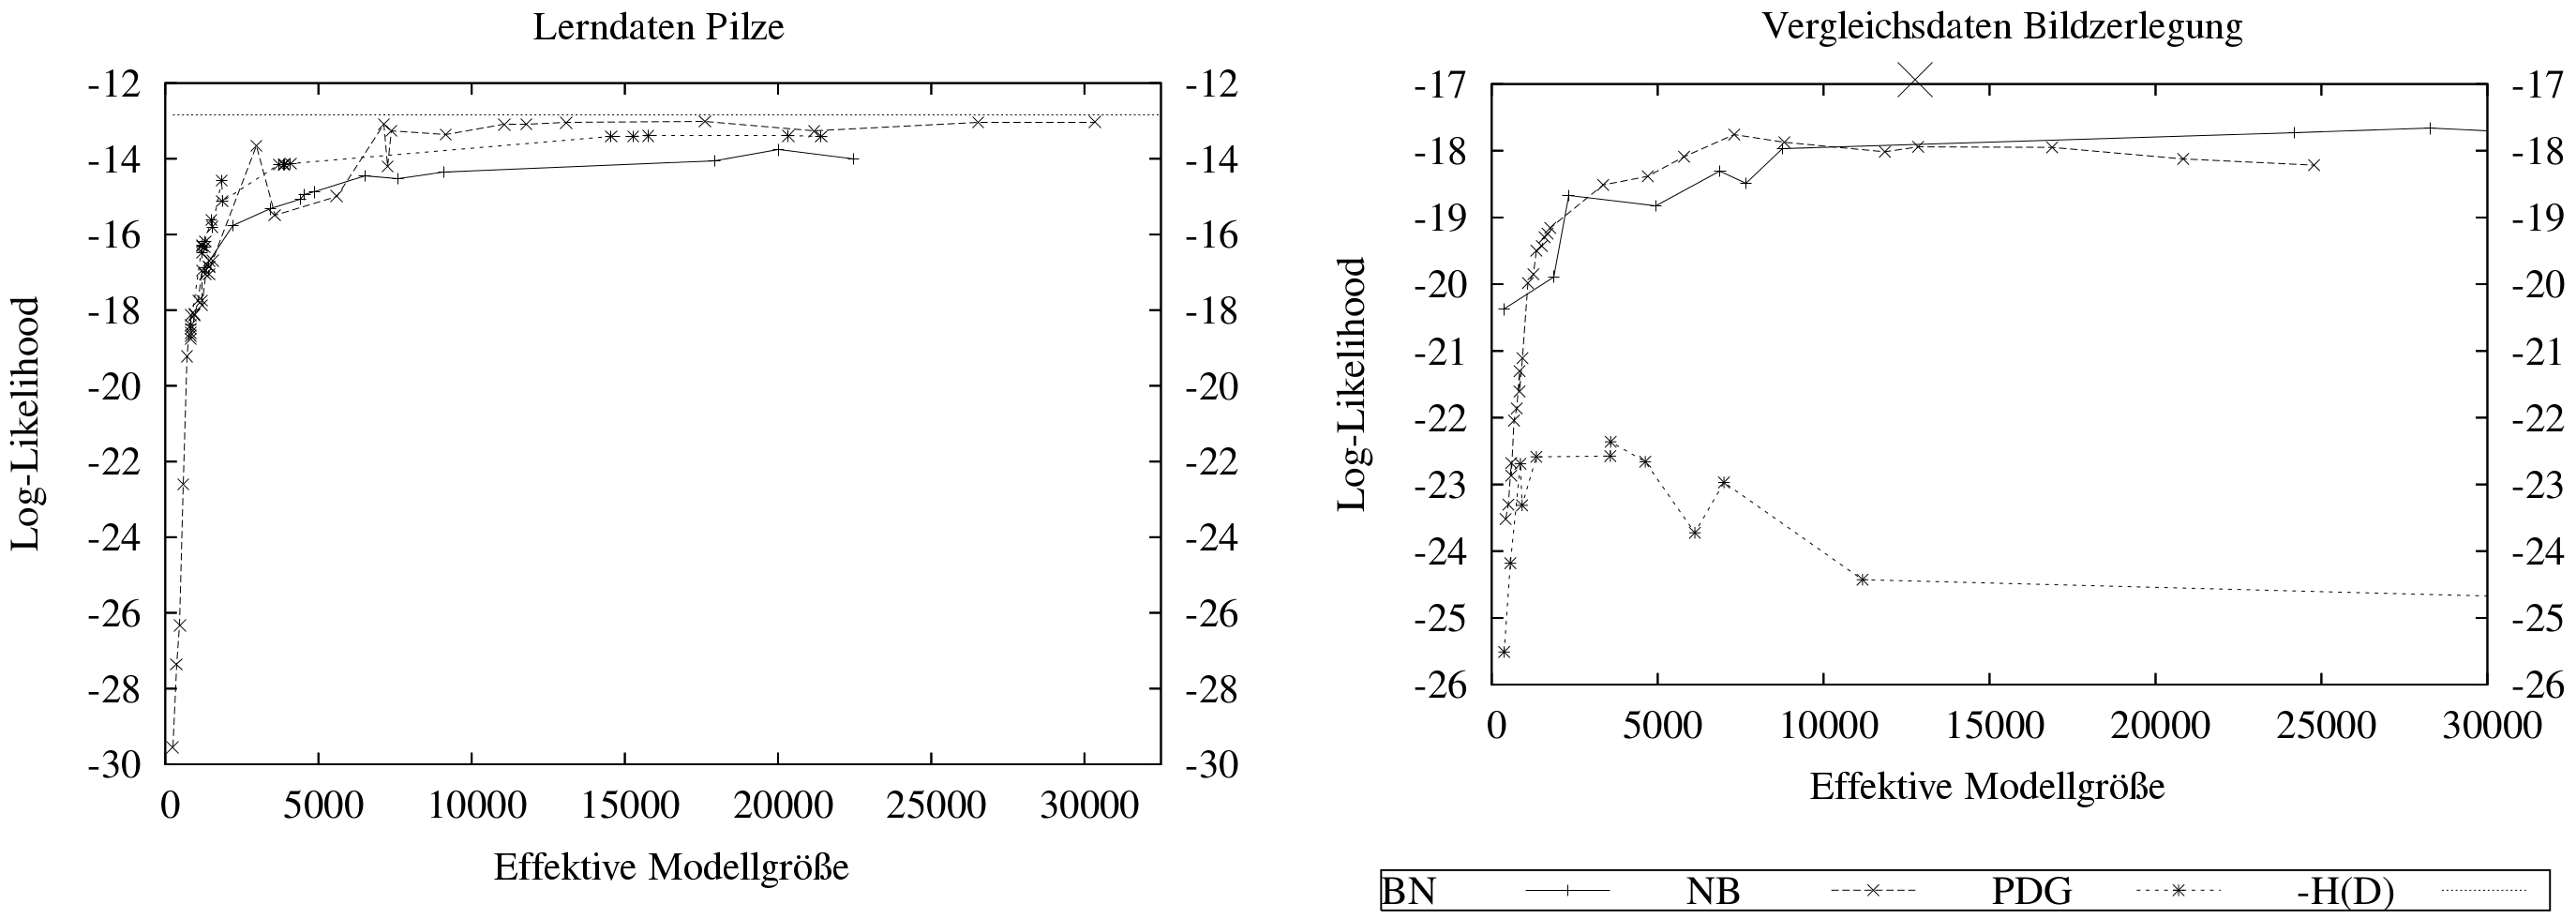
\includegraphics{graphs.png}
  \end{figure}
\end{frame}

\begin{frame}
  \frametitle{Empirische Studie}
  \begin{itemize}
    \item Empirische Messung der Inferenz-Effizienz
    \item Generieren zufälliger Inferenz-Anfragen
    \item Zufällig ausgewählte Menge von Zufallsvariablen
    \item Zufällige Belegungen
    \item Zeit messen
  \end{itemize}
\end{frame}

\begin{frame}
  \frametitle{Zusammenfassung}
  \begin{itemize}
    \item Keine Methode prinzipiell schlechter
    \item NB und PDG teils schneller
    \item NB und PDG leichter zu implementieren
    \item BN in jedem Fall akzeptable Genauigkeit
    \item $\rightarrow$ Für Anwendung im Bereich des Web 2.0 alle in Erwägung ziehen!
  \end{itemize}
\end{frame}


\end{document}
